Para usar InputStick en Bitwarden el usuario deberá instalar la versión modificada de Bitwarden realizada en este proyecto, también deberá realizar la instalación de InputStickUtility. Una vez hecho esto, deberá iniciar sesión o registrarse en Bitwarden o Vaultwarden, así como configurar la clave de InputStick en InputStickUtility. Tras ello en los ajustes puede activar la funcionalidad y la configuración de la misma. Finalmente cuando quiera introducir los credenciales en otro dispositivo simplemente hay que conectar InputStick al dispositivo y acceder al \gls{login} ahí deberá pulsar en el icono de enviar, se le solicitará activar Bluetooth y el campo se escribirá automáticamente en donde se encuentre el foco en el dispositivo. En la figura \ref{fig:diagrama_de_usuario} vemos lo que ocurre a ojos del usuario.

\begin{figure}[H]
    \centering
    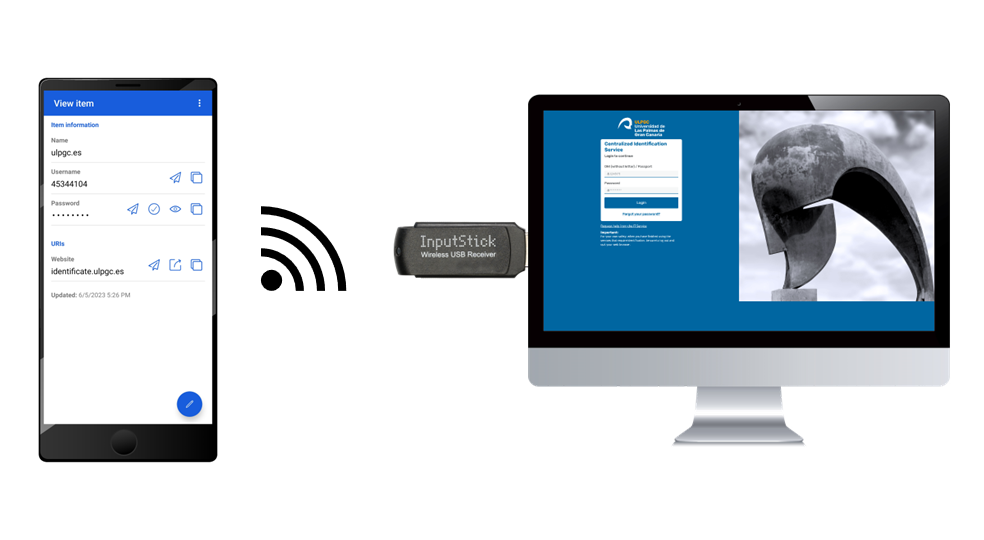
\includegraphics[width=\textwidth]{gfx/diagrama_de_usuario.png}
    \caption{Diagrama de usuario. Realización propia.}
    \label{fig:diagrama_de_usuario}
    El ordenador sobremesa es a modo de ejemplo, pero es sustituible por cualquier dispositivo compatible con \gls{usb} \gls{hid}.\newline
    Marco de móvil. Imagen por brgfx en Freepik.com.\newline
    Marco de monitor. Imagen por d3images en Freepik.com.\newline
\end{figure}